%% Kaplan Business School — Report Template
%% ------------------------------------------------------------------
%% Generic LaTeX template for Overleaf + Git sync.
%% Referencing: Kaplan Harvard Style Guide (v4.0, Feb 2023)
%% ASC Guide to Report Writing compliant
%% ------------------------------------------------------------------

\documentclass[12pt, a4paper]{article}

% ── Encoding & Language ─────────────────────────────────────────────
\usepackage[utf8]{inputenc}
\usepackage[T1]{fontenc}
\usepackage[australian]{babel}          % Australian English spelling

% ── Page Geometry ───────────────────────────────────────────────────
\usepackage[
  top=2.54cm,
  bottom=2.54cm,
  left=2.54cm,
  right=2.54cm
]{geometry}

% ── Fonts ───────────────────────────────────────────────────────────
\usepackage{mathptmx}                   % Times New Roman equivalent
\usepackage{setspace}
\onehalfspacing                         % 1.5 line spacing (academic standard)

% ── Code & Prompt Listings ─────────────────────────────────────────
\usepackage{listings}
\usepackage[dvipsnames]{xcolor}

% Shared colours for code blocks
\definecolor{codebg}{RGB}{245,245,245}
\definecolor{codeframe}{RGB}{200,200,200}
\definecolor{codecomment}{RGB}{106,153,85}
\definecolor{codekeyword}{RGB}{0,0,180}
\definecolor{codestring}{RGB}{163,21,21}
\definecolor{codenumber}{RGB}{130,130,130}

% Base style shared by all listings
\lstdefinestyle{codebase}{
  basicstyle=\ttfamily\footnotesize,
  backgroundcolor=\color{codebg},
  frame=single,
  framesep=6pt,
  rulecolor=\color{codeframe},
  breaklines=true,
  breakatwhitespace=false,
  columns=fullflexible,
  keepspaces=true,
  showstringspaces=false,
  tabsize=4,
  xleftmargin=10pt,
  xrightmargin=10pt,
  aboveskip=10pt,
  belowskip=10pt,
  numbers=left,
  numberstyle=\tiny\color{codenumber},
  numbersep=8pt
}

% Python code style
\lstdefinestyle{python}{
  style=codebase,
  language=Python,
  keywordstyle=\color{codekeyword}\bfseries,
  commentstyle=\color{codecomment}\itshape,
  stringstyle=\color{codestring}
}

% AI prompt style — plain text, no syntax highlighting, no line numbers
\lstdefinestyle{prompt}{
  style=codebase,
  numbers=none,
  basicstyle=\ttfamily\footnotesize\color{black!85}
}

% Default style fallback
\lstset{style=codebase}

% ── Paragraphs ──────────────────────────────────────────────────────
\setlength{\parindent}{0pt}             % No first-line indent
\setlength{\parskip}{6pt}              % Space between paragraphs
\raggedright                            % Left-aligned text (ASC Guide)

% ── Graphics & Figures ──────────────────────────────────────────────
\usepackage{graphicx}
\graphicspath{{figures/}}
\usepackage{float}                      % [H] placement
\usepackage[labelfont=bf]{caption}      % Bold "Figure X:"

% ── Tables ──────────────────────────────────────────────────────────
\usepackage{booktabs}                   % Professional table rules
\usepackage{tabularx}                   % Full-width tables
\usepackage{array}

% ── Acronyms & Glossary ─────────────────────────────────────────────
% Uses noidx mode — no external makeglossaries build step required.
% Works out of the box in Overleaf and local builds alike.
\usepackage[acronyms]{glossaries}
\makenoidxglossaries

% ── Colour & Links ──────────────────────────────────────────────────
% xcolor already loaded above with dvipsnames option
\usepackage[
  colorlinks  = true,
  linkcolor   = NavyBlue,
  citecolor   = NavyBlue,
  urlcolor    = RoyalBlue,
  breaklinks  = true
]{hyperref}
\usepackage{xurl}                       % Better URL line breaks (esp. references)
\Urlmuskip=0mu plus 1mu\relax          % Allow extra URL break opportunities
\emergencystretch=3em                  % Avoid margin overflow in long bibliography lines

% ── Section Formatting ──────────────────────────────────────────────
\usepackage{titlesec}
\titleformat{\section}
  {\normalfont\Large\bfseries}{\thesection}{1em}{}
\titleformat{\subsection}
  {\normalfont\large\bfseries}{\thesubsection}{1em}{}
\titleformat{\subsubsection}
  {\normalfont\normalsize\bfseries}{\thesubsubsection}{1em}{}

% ── Headers & Footers ──────────────────────────────────────────────
\usepackage{fancyhdr}
\setlength{\headheight}{14pt}
\pagestyle{fancy}
\fancyhf{}
\fancyhead[L]{\small\unitcode\ --- \assessmentname}
\fancyhead[R]{\small\thepage}
\fancyfoot[L]{\small\unitcode\ --- \unitname}
\fancyfoot[R]{\small Kaplan Business School - \the\year}
\renewcommand{\headrulewidth}{0.4pt}
\renewcommand{\footrulewidth}{0.2pt}

% ── Harvard Referencing (Kaplan-aligned) ────────────────────────────
\usepackage[round]{natbib}
\bibliographystyle{kaplan-harvard}      % Custom .bst in this repo
\setlength{\bibsep}{0pt}               % Single spacing between refs
\setlength{\bibhang}{1.27cm}           % Hanging indent (standard)

% ── Miscellaneous ──────────────────────────────────────────────────
\usepackage{enumitem}                   % Customisable lists
\usepackage{microtype}                  % Better typography
\usepackage{csquotes}                   % Smart quotes
\usepackage[section]{placeins}          % Keep floats within sections
\usepackage{pdfpages}                   % Include external PDFs (diagrams)
\usepackage[hang,bottom]{footmisc}      % Cleaner, easier-to-read footnotes
\setlength{\skip\footins}{14pt}         % Space before the footnote area
\setlength{\footnotesep}{8pt}           % Space between footnotes
\setlength{\footnotemargin}{1.4em}      % Align wrapped footnote lines neatly
\renewcommand{\footnotelayout}{\footnotesize\setstretch{1.05}\raggedright}
\renewcommand{\footnoterule}{%
  \vspace*{2pt}%
  \noindent\color{black!45}\rule{0.36\textwidth}{0.4pt}%
  \vspace*{5pt}%
}

% ── Word-count helper ──────────────────────────────────────────────
% Run:  texcount -inc -total main.tex

% ════════════════════════════════════════════════════════════════════
%  FILL IN YOUR DETAILS BELOW — these variables populate the entire
%  document (title page, headers, footers) automatically.
% ════════════════════════════════════════════════════════════════════
\newcommand{\unitcode}{TECH2100}
\newcommand{\unitname}{Introduction to Information Networks}
\newcommand{\assessmentname}{Assessment 1}
\newcommand{\reporttitle}{Report Evaluation}
\newcommand{\studentname}{Patrick de Freitas}
\newcommand{\studentid}{1885133}
\newcommand{\trimester}{TX 20XX}
\newcommand{\campusname}{KBS Perth}
\newcommand{\lecturername}{Lecturer Name}

% ════════════════════════════════════════════════════════════════════
%  DEFINE ACRONYMS HERE
%  First use in text:       \acrfull{key}  → Full Name (ABR)
%  Subsequent uses:         \acrshort{key} → ABR
%  Example:
%  \newacronym{zta}{ZTA}{Zero Trust Architecture}
% ════════════════════════════════════════════════════════════════════


% ────────────────────────────────────────────────────────────────────
%                         DOCUMENT START
% ────────────────────────────────────────────────────────────────────
\begin{document}

% ═══════════════════════════════════════════════════════════════════
%  TITLE PAGE
% ═══════════════════════════════════════════════════════════════════
\begin{titlepage}
  \centering
  \vspace*{2cm}

  {\LARGE\bfseries \unitcode\ --- \unitname\\[6pt]}
  {\Large \assessmentname\\[24pt]}

  \rule{\textwidth}{1pt}\\[18pt]

  {\huge\bfseries \reporttitle\\[18pt]}

  \rule{\textwidth}{1pt}\\[36pt]

  {\Large
    \textbf{Student Name:} \studentname\\[6pt]
    \textbf{Student ID:}   \studentid\\[6pt]
    \textbf{Campus:}       \campusname\\[6pt]
  }

  \vfill
  {\large Kaplan Business School\\[6pt]}
  {\large Master of Information Technology\\[6pt]}
  {\large \today}
\end{titlepage}

% ═══════════════════════════════════════════════════════════════════
%  FRONT MATTER — Roman numeral pagination (ASC Guide)
% ═══════════════════════════════════════════════════════════════════
\pagenumbering{roman}
\setcounter{page}{2}                    % Title page is implicitly page i

% ═══════════════════════════════════════════════════════════════════
%  TABLE OF CONTENTS
% ═══════════════════════════════════════════════════════════════════
\newpage
\tableofcontents
\newpage

% ═══════════════════════════════════════════════════════════════════
%  EXECUTIVE SUMMARY (ASC Guide — separate page, written last)
% ═══════════════════════════════════════════════════════════════════
\section*{Executive Summary}
\addcontentsline{toc}{section}{Executive Summary}
\label{sec:executive-summary}

\textit{[Write this section last. It should be half to three-quarters
of a page (50--300 words) and include:
the purpose and a brief description of the research;
a summary of the findings and conclusions;
a summary of the key recommendations.]}

\newpage

% ═══════════════════════════════════════════════════════════════════
%  BODY — Switch to Arabic page numbering
% ═══════════════════════════════════════════════════════════════════
\pagenumbering{arabic}

% ═══════════════════════════════════════════════════════════════════
%  CITATION CHEAT SHEET (delete before submission)
% ═══════════════════════════════════════════════════════════════════
% Parenthetical:  \citep{key}              → (Author Year)
% Textual:        \citet{key}              → Author (Year)
% With page:      \citep[p.~42]{key}       → (Author Year, p. 42)
% Multiple:       \citep{key1,key2}        → (Author1 Year; Author2 Year)
% No brackets:    \citealt{key}            → Author Year
% In caption:     (adapted from \citealt{key})

% ═══════════════════════════════════════════════════════════════════
%  1. INTRODUCTION (ASC Guide — background, purpose, scope)
% ═══════════════════════════════════════════════════════════════════
\section{Introduction}
\label{sec:introduction}

\textit{[Background: Briefly describe the context and identify the
general subject matter indicating why the report was commissioned.]}

\textit{[Purpose: Describe the issue(s) or problem(s) to be reported
on and what the report hopes to accomplish.]}

\textit{[Scope: Outline what issues are covered in the report and
what issues are not covered. Also known as the brief or terms of
reference.]}

% ═══════════════════════════════════════════════════════════════════
%  2. SECTION TWO
% ═══════════════════════════════════════════════════════════════════
\section{Potential reputation, financial and legal loss of current network architecture}
\label{sec:section-one}

Along the years, technologies have been experiencing a rapidly evolution and it close to what is known as Moore's law. Intel co-founder Gordon Moore predicted a doubling of transistors every year for the next 10 years in his original paper published in 1965. This boom in the evolution is followed by its demand adding extra stress to the network infrastructure and a major outage in entire Australia could potentially cause a damage of AUD \$29,828,489 per hour (Figure 01).

Figure 01: Data from the Netblocks, the economic impact of a single hypothetical internet disruption of the specified type, location and duration.


% ═══════════════════════════════════════════════════════════════════
%  3. SECTION THREE
% ═══════════════════════════════════════════════════════════════════
\section{Section Three}
\label{sec:section-three}

\subsection{Subsection A}
\label{subsec:three-a}

Maecenas sed diam eget risus varius blandit sit amet non magna. Integer
posuere erat a ante venenatis dapibus posuere velit aliquet
\citep{Zhang2020}. Praesent commodo cursus magna, vel scelerisque nisl
consectetur et.

\subsection{Subsection B --- Figure Example}
\label{subsec:three-b}

% Place your diagram(s) in the figures/ folder:
\begin{figure}[H]
  \centering
  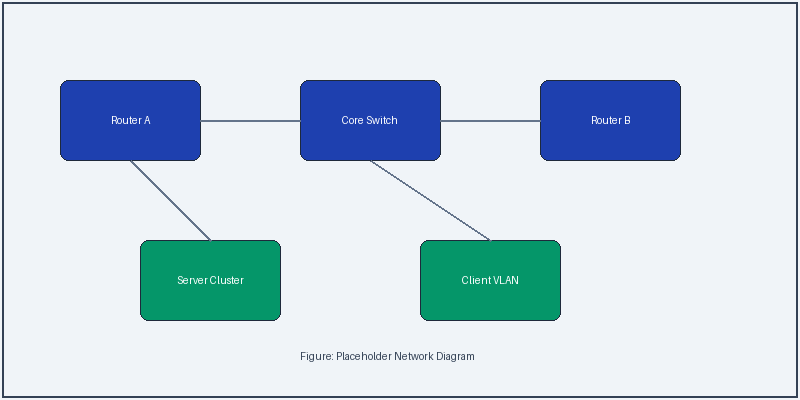
\includegraphics[width=0.85\textwidth]{dummy_network_diagram.png}
  \caption{Placeholder diagram showing a sample layout
           (adapted from \citealt{Kurose2021}).}
  \label{fig:sample-diagram}
\end{figure}

As shown in Figure~\ref{fig:sample-diagram}, the layout separates
components into distinct layers. \citet{Tanenbaum2021} recommend
this approach for medium-scale deployments.

\subsection{Subsection C}
\label{subsec:three-c}

Fusce dapibus, tellus ac cursus commodo, tortor mauris condimentum nibh,
ut fermentum massa justo sit amet risus \citep{Kreutz2015}.


% ═══════════════════════════════════════════════════════════════════
%  4. SECTION FOUR
% ═══════════════════════════════════════════════════════════════════
\section{Section Four}
\label{sec:section-four}

\subsection{Subsection A}
\label{subsec:four-a}

Etiam porta sem malesuada magna mollis euismod. Vivamus sagittis lacus
vel augue laoreet rutrum faucibus dolor auctor \citep{Cisco2020}.

\subsection{Subsection B}
\label{subsec:four-b}

Cum sociis natoque penatibus et magnis dis parturient montes, nascetur
ridiculus mus \citep{IEEE802.3}. Donec ullamcorper nulla non metus
auctor fringilla.

\subsection{Subsection C}
\label{subsec:four-c}

Sed posuere consectetur est at lobortis. Cras justo odio, dapibus ut
facilisis in, egestas eget quam \citep{Akyildiz2010}.


% ═══════════════════════════════════════════════════════════════════
%  5. SECTION FIVE
% ═══════════════════════════════════════════════════════════════════
\section{Section Five}
\label{sec:section-five}

\subsection{Subsection A}
\label{subsec:five-a}

Maecenas faucibus mollis interdum. Duis mollis, est non commodo luctus,
nisi erat porttitor ligula, eget lacinia odio sem nec elit
\citep{Floridi2018}. Nullam id dolor id nibh ultricies vehicula ut id
elit.

\subsection{Subsection B}
\label{subsec:five-b}

Aenean eu leo quam. Pellentesque ornare sem lacinia quam venenatis
vestibulum. Donec id elit non mi porta gravida at eget metus
\citep{NIST2020}.

\subsection{Subsection C}
\label{subsec:five-c}

Vivamus sagittis lacus vel augue laoreet rutrum faucibus dolor auctor.
Cras mattis consectetur purus sit amet fermentum \citep{Boutaba2018}.


% ═══════════════════════════════════════════════════════════════════
%  6. CONCLUSION
% ═══════════════════════════════════════════════════════════════════
\section{Conclusion}
\label{sec:conclusion}

Donec sed odio dui. Etiam porta sem malesuada magna mollis euismod.
Nullam quis risus eget urna mollis ornare vel eu leo. Integer posuere
erat a ante venenatis dapibus posuere velit aliquet.


% ═══════════════════════════════════════════════════════════════════
%  7. RECOMMENDATIONS (ASC Guide — separate from Conclusion)
% ═══════════════════════════════════════════════════════════════════
\section{Recommendations}
\label{sec:recommendations}

\textit{[Provide clear, actionable recommendations based on the
findings and conclusions presented in the report. Each recommendation
should be specific and justified by the evidence discussed in the
body of the report.]}


% ═══════════════════════════════════════════════════════════════════
%  REFERENCE LIST
% ═══════════════════════════════════════════════════════════════════
% Kaplan Harvard rules:
%   - Heading: "Reference List"
%   - Alphabetical by first author surname
%   - Left justified, single spacing, same font as body
%   - Hanging indent
%   - Minimal capitalisation (first word + proper nouns only)
\newpage
\renewcommand{\refname}{Reference List}
\bibliography{references}


% ═══════════════════════════════════════════════════════════════════
%  APPENDICES (optional — typically not counted in word limit)
%  Numbered A1, A2, A3...  Pair prompts with response screenshots.
%  Usage:
%    \begin{lstlisting}[style=prompt] ... \end{lstlisting}
%    \begin{lstlisting}[style=python] ... \end{lstlisting}
% ═══════════════════════════════════════════════════════════════════
\newpage
\appendix
\renewcommand{\thesection}{A\arabic{section}}

\section{Diagrams}
\label{app:diagrams}

\textit{[Include full-size diagrams here if needed.]}

\section{Supporting Material}
\label{app:supporting}

\textit{[Include supporting material here.]}

\section{Prompt - Example}
\label{app:a3-prompt}

\textit{[Document Generative AI prompts used. Include model name.]}

% \textbf{Model:} Claude / ChatGPT / etc.
%
% \begin{lstlisting}[style=prompt]
% Your prompt text here.
% \end{lstlisting}


% ═══════════════════════════════════════════════════════════════════
%  LIST OF ABBREVIATIONS — auto-populated from \newacronym definitions
% ═══════════════════════════════════════════════════════════════════
\newpage
\printnoidxglossary[type=\acronymtype, title=List of Abbreviations]

% ═══════════════════════════════════════════════════════════════════
%  GLOSSARY — add terms with \newglossaryentry{key}{name=...,description=...}
% ═══════════════════════════════════════════════════════════════════
\printnoidxglossary[title=Glossary]

\end{document}
